\chapter{Implementacja i opis projektu}

W niniejszym rozdziale przedstawiono sposób implementacji systemu wspomagającego trening oddechowy. Opis ten  obejmuje pochodzenie projektu jakim jest kontynuacja wybranych prac. Omówione zostały wybrane technologie oraz podział odpowiedzialności pomiędzy modułami. Przedstawiony zostanie również przepływ danych od rejestracji dźwięku do prezentacji wyniku użytkownikowi. Głównym założeniem architektonicznym było oddzielenie wieloplatformowej aplikacji mobilnej od procesu uczenia modelu. Model był rozwijany w środowisku Python z pomocą biblioteki PyTorch, a następnie został wyeksportowany do formatu ONNX, który został dołączony do aplikacji Flutter.

\section{Geneza i zakres projektu}

Opracowany system stanowi kontynuację dwóch wcześniejszych projektów. Pierwszym z~nich jest \textit{ReSpire}, czyli aplikacja mobilna przygotowana we frameworku Flutter i języku Dart dla systemów Android oraz iOS \cite{respireGithub2026}. Repozytorium projektu zawiera wydzielone katalogi odpowiedzialne między innymi za komponenty interfejsu, widoki, usługi, motyw graficzny, a także funkcje pomocnicze. Struktura ta stała się podstawą warstwy aplikacyjnej rozwijanej w ramach niniejszej pracy.

W stosunku do pierwotnej wersji ReSpire wprowadzano iteracyjne udoskonalenia interfejsu użytkownika. Prace koncentrowały się na dopracowaniu prezentacji treningu i ogólnej poprawie doświadczenia użytkownika z daną aplikacją.  Oprócz tego dodane zostały opcje rozszerzające możliwości personalizacji treningów oraz interfejs został przygotowany do wyświetlania wyniku klasyfikacji w czasie rzeczywistym. Skorzystanie z istniejącej bazy aplikacji pozwoliło skupić dalszy rozwój na integracji z modułem uczenia maszynowego, bez konieczności ponownego tworzenia podstawowej nawigacji, jak również warstwy wizualnej.

Drugim projektem jest \textit{breathing-classification-v2}, zawierający narzędzia do zbierania i przetwarzania danych, implementacje modeli, skrypty treningowe, mechanizmy ewaluacji oraz aplikację demonstracyjną \cite{breathingClassificationGithub2026}. W projekcie tym rozwijano kilka sposobów klasyfikacji oddechu, w tym modele LSTM, modele analizujące widmo oraz architekturę transformerową. W niniejszej pracy wykorzystano rozwiązania rozwijane w wariancie określanym jako \texttt{exhale\_detection}, który stanowił punkt wyjścia dla detekcji wydechu i integracji klasyfikatora z aplikacją.

Obecny projekt łączy obie linie rozwojowe. Z ReSpire przejęto podstawową architekturę aplikacji, a także interfejs, natomiast z projektu klasyfikacji oddechu wykorzystano potok przetwarzania dźwięku, model CNN-Transformer oraz mechanizm eksportu do ONNX. W efekcie powstał system, w którym aplikacja odpowiada za obsługę użytkownika i rejestrację dźwięku, a wydzielony model za wykrywanie wydechu wykorzystywane do zliczania cykli oddechowych.

\medskip
\noindent\textbf{Aplikacja ReSpire}\par
\noindent Projekt bazowy: \url{https://github.com/GGBJacob/ReSpire}\par
\noindent Wersja rozwijana: \url{https://github.com/PCyganiuk/ReSpire}

\medskip
\noindent\textbf{Model klasyfikacji oddechu}\par
\noindent Projekt bazowy: \url{https://github.com/peterprospl12/breathing-classification-v2}\par
\noindent Wersja rozwijana: \url{https://github.com/PCyganiuk/breathing-classification-v3}

\newpage
\section{Przypadki użycia aplikacji}

Model przypadków użycia przedstawia najważniejsze funkcje aplikacji z perspektywy użytkownika końcowego oraz zależności pomiędzy nimi. Jego celem jest pokazanie, jakie działania użytkownik może wykonać podczas zarządzania treningami oddechowymi i konfiguracji aplikacji. Na diagramie pominięto szczegóły implementacyjne, takie jak zapis danych, komunikacja z natywną warstwą systemu czy uruchamianie modelu detekcji. Elementy te są obsługiwane wewnętrznie i nie wymagają bezpośredniej interakcji użytkownika.

\begin{figure}[H]
    \centering
    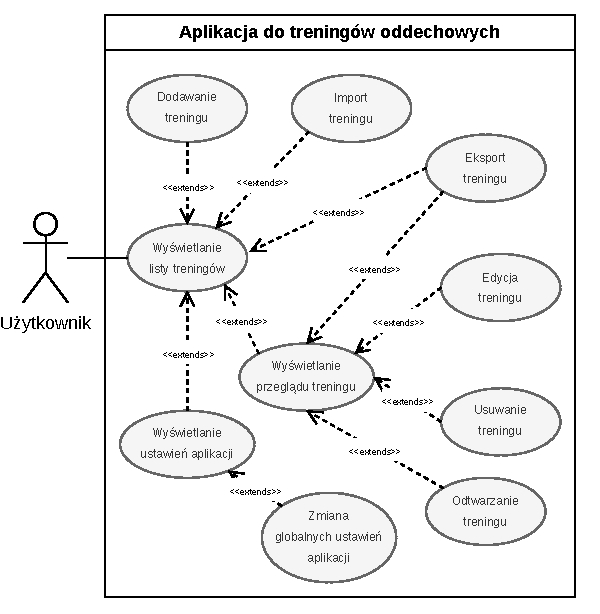
\includegraphics[width=0.90\linewidth,height=0.78\textheight,keepaspectratio]{obrazy/use_case.drawio-1.pdf}
    \caption{Diagram przypadków użycia aplikacji ReSpire}
    \label{fig:use_case_diagram}
\end{figure}

Jedynym aktorem przedstawionym na diagramie jest użytkownik aplikacji. Podstawowym przypadkiem użycia jest \textbf{Wyświetlanie listy treningów}, stanowiące główny punkt dostępu do pozostałych funkcji. Z tego miejsca użytkownik może wykonać przypadki: \textbf{Dodawanie treningu}, \textbf{Import treningu}, \textbf{Eksport treningu} albo \textbf{Wyświetlanie przeglądu treningu}. Zastosowane na diagramie relacje \textit{extend} wskazują działania opcjonalne, które rozszerzają podstawowy przebieg pracy z listą i są wykonywane dopiero po zgłoszeniu odpowiedniego żądania przez użytkownika.

\newpage

Przypadek \textbf{Dodawanie treningu} umożliwia zdefiniowanie jego nazwy, etapów, grup, liczby powtórzeń oraz parametrów poszczególnych faz oddechu. Po zatwierdzeniu poprawnie utworzony trening jest zapisywany i pojawia się na liście. \textbf{Import treningu} pozwala wczytać jeden lub kilka treningów z pliku o obsługiwanym formacie. Przed zapisem aplikacja powinna sprawdzić poprawność struktury danych, a w przypadku błędnego pliku przerwać operację i wyświetlić odpowiedni komunikat. \textbf{Eksport treningu} realizuje działanie odwrotne: dane treningu są przekształcane do postaci możliwej do zapisania i późniejszego ponownego zaimportowania.

Po wybraniu elementu z listy wykonywany jest przypadek \textbf{Wyświetlanie przeglądu treningu}. Ekran ten przedstawia jego strukturę, czasy faz, przyrosty oraz kolejność grup, dzięki czemu ustawienia mogą zostać sprawdzone przed rozpoczęciem ćwiczenia. Z poziomu przeglądu dostępne są trzy dalsze przypadki: \textbf{Edycja treningu}, \textbf{Usuwanie treningu} i \textbf{Odtwarzanie treningu}. Edycja pozwala zmienić istniejącą konfigurację i zapisać jej nową postać. Usuwanie wymaga potwierdzenia, ponieważ prowadzi do usunięcia treningu z lokalnych danych aplikacji. Odtwarzanie rozpoczyna sesję zgodnie z zapisanym wzorcem i uruchamia wybrane formy prowadzenia ćwiczenia, takie jak wizualizacja lub wskazówki dźwiękowe. Jeżeli monitorowanie za pomocą mikrofonu jest aktywne, podczas treningu może być również wykorzystywany moduł wykrywania wydechu.

Osobną grupę stanowią przypadki \textbf{Wyświetlanie ustawień aplikacji} i \textbf{Zmiana globalnych ustawień aplikacji}. Użytkownik może otworzyć widok ustawień i zmienić parametry obowiązujące globalnie, niezależnie od konfiguracji konkretnego treningu. Obejmują one między innymi sposób prezentowania ćwiczenia, zachowanie ekranu oraz ustawienia funkcji monitorujących. Oddzielenie ustawień globalnych od parametrów treningu ogranicza konieczność powtarzalnego konfigurowania tych samych opcji dla każdej sesji.

\section{Architektura rozwiązania}

System został podzielony na warstwę prezentacji, logikę aplikacji, moduł przetwarzania dźwięku oraz moduł wnioskowania. Taki podział ogranicza zależności pomiędzy interfejsem a modelem. Umożliwia również wymianę pliku ONNX bez przebudowy całej aplikacji oraz testowanie klasyfikatora niezależnie od warstwy wizualnej.

Warstwa Flutter odpowiada za interfejs i logikę aplikacji, natomiast uruchamianie modelu odbywa się w kodzie natywnym. Komunikacja pomiędzy kodem Dart a warstwami platformowymi jest realizowana za pomocą kanałów platformowych \cite{flutterPlatformChannels2026}. W zrealizowanej integracji BCV3 aplikacja przekazuje przygotowane dane wejściowe do modułu Kotlin w systemie Android. Kod natywny uruchamia model za pomocą ONNX Runtime, a następnie zwraca do Fluttera wynik detekcji wydechu. Warstwa aplikacyjna jest przygotowana również dla systemu iOS, jednak natywna integracja BCV3 w module Swift nie została przeprowadzona, przy czym pozostaje kierunkiem dalszych prac. Schemat architektury przedstawiono na rysunku \ref{fig:implementation_pipeline}; ścieżka dla iOS stanowi docelowy wariant integracji.

\begin{figure}[H]
    \centering
    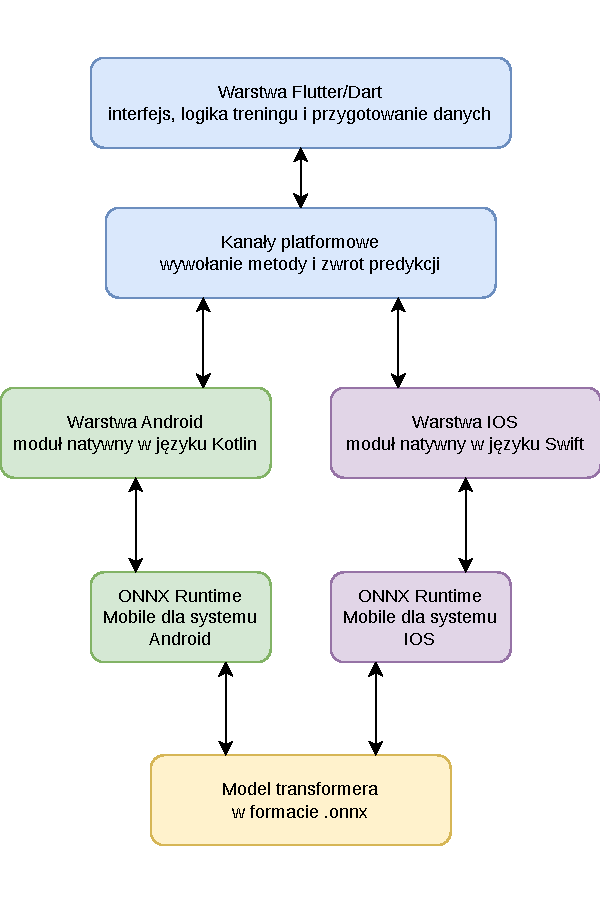
\includegraphics[width=0.82\linewidth,height=0.5\textheight,keepaspectratio]{obrazy/flow_diagram.pdf}
    \caption{Komunikacja warstwy Flutter z natywnymi modułami uruchamiającymi model ONNX}
    \label{fig:implementation_pipeline}
\end{figure}

Rozdzielenie etapu treningu i wnioskowania ma również znaczenie praktyczne. Proces uczenia może wykorzystywać komputer wyposażony w procesor graficzny, większą ilość pamięci oraz pełne środowisko PyTorch. Aplikacja końcowa zawiera wyłącznie model przeznaczony do predykcji i lekkie środowisko wykonawcze. Dzięki temu urządzenie mobilne nie musi udostępniać bibliotek używanych podczas trenowania.

\section{Warstwa aplikacyjna we Flutterze}

Do implementacji aplikacji wybrano Flutter, który umożliwia tworzenie interfejsu i logiki dla wielu platform z wykorzystaniem języka Dart oraz wspólnej bazy kodu \cite{flutterDocs2026}. Wybór tej technologii wynikał również z faktu, że wcześniejszy projekt ReSpire został już przygotowany we Flutterze. Kontynuowanie tej architektury ograniczyło koszt migracji, przy czym pozwoliło zachować istniejące komponenty.

Do rozwoju i testowania aplikacji mobilnej wykorzystano środowisko Android Studio. Zapewniało ono kompleksowe wsparcie dla kodu Flutter oraz Dart, jak i zarządzanie konfiguracją projektu dla systemu Android. Dzięki niemu możliwe było również uruchamianie aplikacji na emulatorze oraz podłączonym urządzeniu, a także analizowanie komunikatów diagnostycznych i błędów pojawiających się podczas działania aplikacji. Środowisko było również wykorzystywane podczas integracji warstwy Flutter z natywnym kodem Kotlin i biblioteką ONNX Runtime.

Warstwa Flutter odpowiada za uruchamianie sesji treningowej, obsługę uprawnień do mikrofonu, przechwytywanie danych, prezentację wyniku detekcji, a także sterowanie animacjami. Kod aplikacji został rozdzielony na elementy interfejsu, strony, usługi i funkcje pomocnicze. Komponenty wizualne mogą dzięki temu być modyfikowane niezależnie od kodu obsługującego dźwięk oraz model.

Z punktu widzenia interfejsu wynik modelu jest stanem aplikacji. Po otrzymaniu predykcji odpowiednie elementy ekranu są aktualizowane, aby wskazać wykrycie wydechu, który sygnalizuje koniec cyklu oddechowego. Ten sam wynik jest używany również do zliczania cykli i wyświetlenia odpowiedniej informacji o przebiegu treningu po jego zakończeniu. Interfejs nie musi znać szczegółów architektury sieci neuronowej, ponieważ otrzymuje jedynie etykietę oraz wartości wyjściowe modelu.

Wieloplatformowość Fluttera umożliwia utrzymywanie wspólnej logiki dla kolejnych systemów docelowych. Elementy zależne od platformy, takie jak konfiguracja uprawnień, sposób dostępu do mikrofonu lub integracja natywnego środowiska ONNX, mogą być wydzielone do odpowiednich katalogów platformowych albo obsłużone przez wtyczki. Pozwala to rozwijać wersje aplikacji bez duplikowania całej warstwy prezentacji.

\subsection{Diagram klas treningu}

Diagram klas przedstawia model danych wykorzystywany do zapisu konfiguracji treningu, ustawień sesji i przypisanych dźwięków. Pokazuje on zarówno hierarchię obiektów tworzących trening, jak i klasy pomocnicze odpowiedzialne za personalizację poszczególnych faz. Na diagramie wskazano również pliki źródłowe projektu, w których zawarto definicje poszczególnych klas. Aktualną postać modelu przedstawiono na rysunku \ref{fig:training_class_diagram}.

\begin{landscape}
\begin{figure}[H]
    \centering
    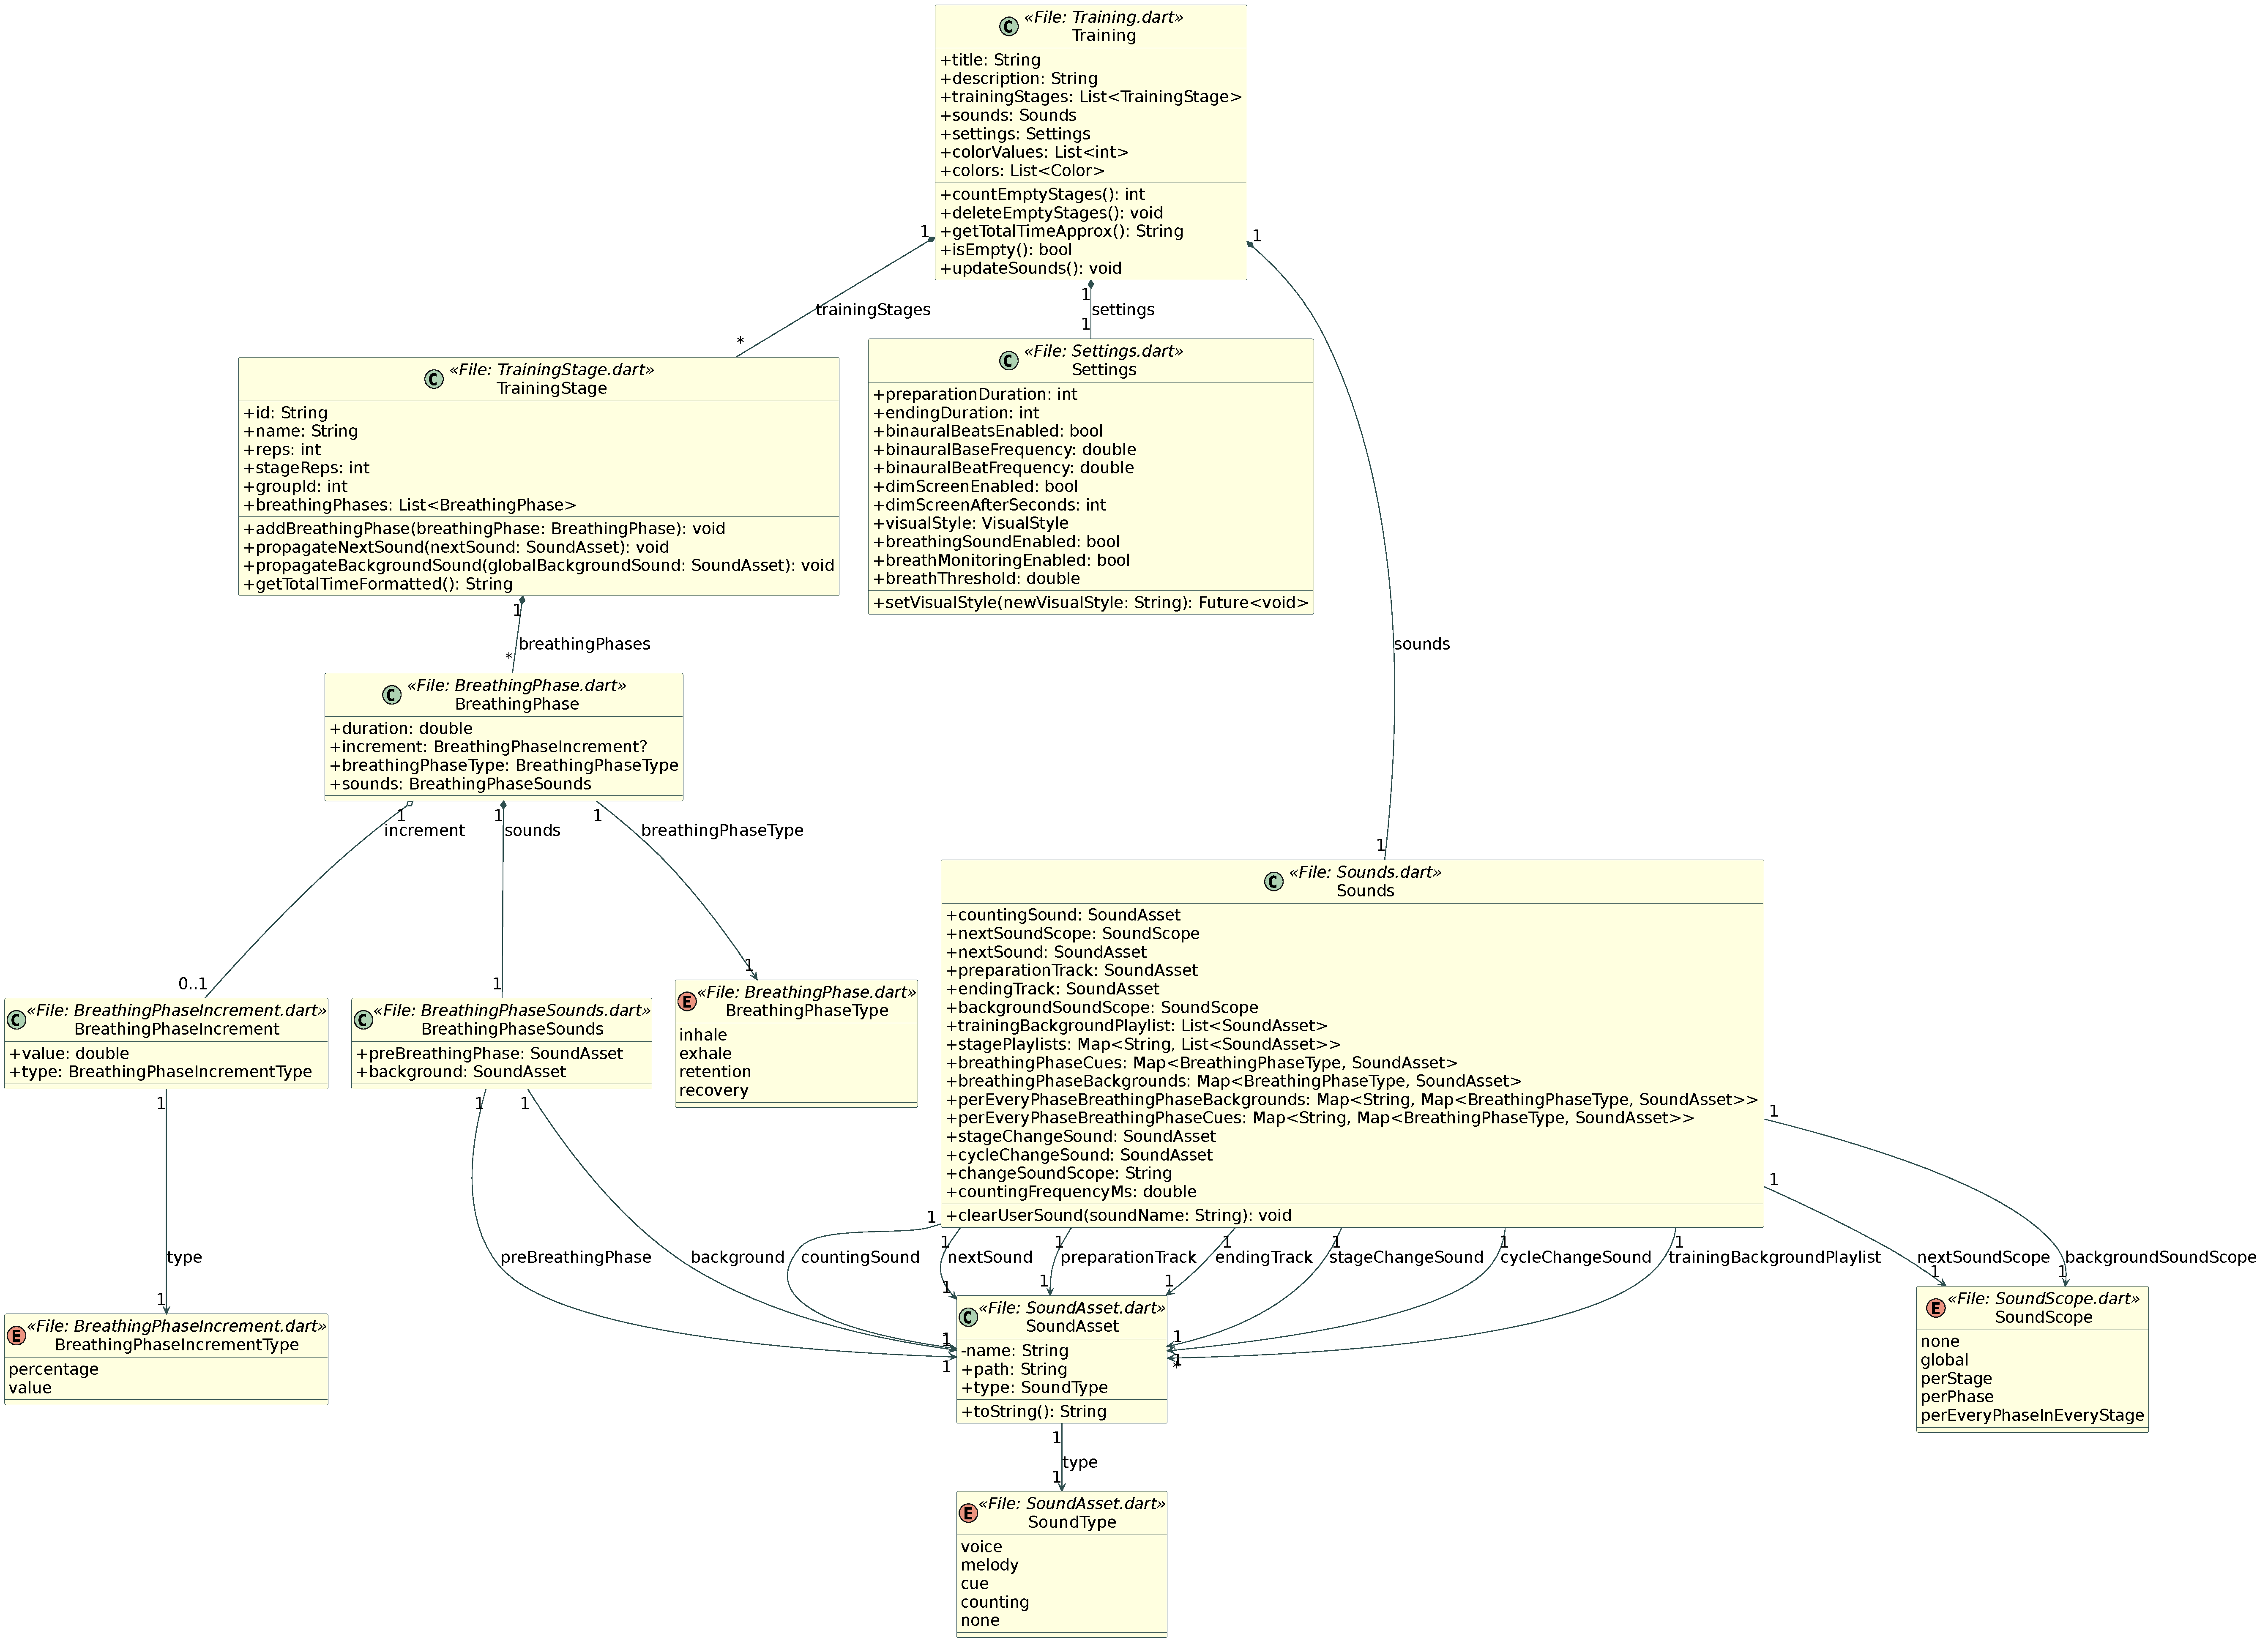
\includegraphics[width=\textheight,height=0.95\textwidth,keepaspectratio]{obrazy/use_case_files-1.pdf}
    \caption{Diagram klas modelu treningu aplikacji ReSpire}
    \label{fig:training_class_diagram}
\end{figure}
\end{landscape}

\subsection{Struktura danych treningu}

Model danych treningu ma strukturę hierarchiczną, której podstawę tworzą klasy \texttt{Training}, \texttt{TrainingStage}i \texttt{BreathingPhase}. Obiekt \texttt{Training} zawiera listę co najmniej jednego etapu, natomiast każdy etap składa się z uporządkowanej sekwencji faz \texttt{BreathingPhase}. Etapy mogą być dodatkowo łączone w grupy. Elementy należące do tej samej grupy są wykonywane kolejno, po czym cała grupa zostaje powtórzona zadaną liczbę razy. Dopiero po wykonaniu wszystkich powtórzeń aplikacja przechodzi do następnej grupy lub niezgrupowanego etapu.

Klasa \texttt{Training} przechowuje tytuł i opis treningu, listę etapów, ustawienia, konfigurację dźwięków oraz wartości kolorów wykorzystywane do wizualnego rozróżniania grup. Udostępnia również metody pomocnicze służące do wykrywania i usuwania pustych etapów, sprawdzania poprawności struktury, przybliżonego obliczania całkowitego czasu sesji oraz aktualizowania konfiguracji dźwiękowej. Pole \texttt{description} umożliwia uzupełnienie treningu o dodatkowy opis, natomiast \texttt{colorValues} i \texttt{colors} przechowują reprezentację kolorów w postaci możliwej do zapisania oraz obiekty wykorzystywane bezpośrednio przez interfejs.

Obiekt \texttt{TrainingStage} opisuje pojedynczy etap treningu. Oprócz identyfikatora, nazwy i listy faz zawiera pola \texttt{reps}, \texttt{stageReps} oraz \texttt{groupId}. Pole \texttt{reps} określa liczbę cykli wykonywanych wewnątrz etapu, natomiast \texttt{groupId} pozwala przypisać kilka etapów do wspólnej, uporządkowanej grupy. Pole \texttt{stageReps} określa liczbę powtórzeń całej grupy etapów. Klasa etapu nie przechowuje parametru przyrostu czasu, ponieważ progresja jest definiowana niezależnie dla każdej fazy oddechowej. \texttt{TrainingStage} umożliwia ponadto dodawanie faz, obliczanie łącznego czasu etapu oraz propagowanie dźwięku tła i sygnału kolejnej fazy do elementów podrzędnych.

Klasa \texttt{BreathingPhase} reprezentuje pojedynczą czynność oddechową. Pole \texttt{duration} określa jej podstawowy czas trwania, \texttt{breathingPhaseType} wskazuje rodzaj fazy, a \texttt{sounds} przechowuje jej oprawę dźwiękową. Typ wyliczeniowy \texttt{BreathingPhaseType} obejmuje wdech (\texttt{inhale}), wydech (\texttt{exhale}), zatrzymanie oddechu (\texttt{retention}) i regenerację (\texttt{recovery}). Każda faza może mieć własne, opcjonalne pole \texttt{increment}, dzięki czemu czas wdechu, wydechu, zatrzymania lub regeneracji może zmieniać się niezależnie w kolejnych cyklach.

Klasa \texttt{BreathingPhaseIncrement} odpowiada za zmianę czasu trwania konkretnej fazy wraz z kolejnymi powtórzeniami. Zawiera wartość \texttt{value} oraz sposób jej interpretacji określany przez \texttt{BreathingPhaseIncrementType}. Model obsługuje przyrost o wartość bezwzględną (\texttt{value}) oraz zmianę procentową (\texttt{percentage}). Pozwala to przykładowo stopniowo wydłużać wydech, nie zmieniając jednocześnie czasu pozostałych faz w tym samym etapie.

Globalne parametry sesji agreguje klasa \texttt{Settings}. Obejmuje ona czasy przygotowania i zakończenia, konfigurację dźwięków binauralnych, opcję wygaszania ekranu i czas bezczynności poprzedzający wygaszenie. Pole \texttt{visualStyle} wskazuje wybrany sposób wizualizacji treningu. Pola \texttt{breathingSoundEnabled}, \texttt{breathMonitoringEnabled} i \texttt{breathThreshold} sterują odpowiednio dźwiękowym prowadzeniem oddechu, działaniem modułu monitorowania oraz wartością progu detekcji. Metoda \texttt{setVisualStyle()} umożliwia aktualizację stylu wizualizacji wraz z zapisaniem zmiany.

Konfiguracja dźwięków została rozdzielona pomiędzy kilka powiązanych klas:

\begin{itemize}
    \item \texttt{Sounds} jest głównym kontenerem oprawy dźwiękowej treningu. Przechowuje dźwięk odliczania, utwory przygotowania oraz zakończenia, sygnały zmiany etapu i cyklu, globalną listę muzyki, a także listy przypisane do poszczególnych etapów. Mapy faz umożliwiają niezależne określenie sygnałów oraz dźwięków tła dla wdechu, wydechu, zatrzymania i regeneracji. Dodatkowe mapy indeksowane identyfikatorem etapu obsługują osobne ustawienia dla każdej fazy w każdej grupie. Pole \texttt{countingFrequencyMs} określa częstotliwość odtwarzania odliczania;
    \item \texttt{BreathingPhaseSounds} zawiera zasoby związane z pojedynczą fazą: sygnał \texttt{preBreathingPhase} odtwarzany przed jej rozpoczęciem oraz dźwięk \texttt{background} aktywny w czasie trwania fazy;
    \item \texttt{SoundAsset} reprezentuje pojedynczy zasób audio. Przechowuje jego nazwę, ścieżkę oraz kategorię wskazywaną przez \texttt{SoundType};
    \item \texttt{SoundType} rozróżnia głos lektora (\texttt{voice}), melodię (\texttt{melody}), krótki sygnał (\texttt{cue}), odliczanie (\texttt{counting}) i brak dźwięku (\texttt{none});
    \item \texttt{SoundScope} określa zakres obowiązywania dźwięku. Dostępne wartości oznaczają brak przypisania (\texttt{none}), ustawienie globalne (\texttt{global}), przypisanie do etapu (\texttt{perStage}), fazy (\texttt{perPhase}) albo każdej fazy w każdym etapie (\texttt{perEveryPhaseInEveryStage}).
\end{itemize}

Takie rozdzielenie odpowiedzialności pozwala zapisywać zarówno proste treningi wykorzystujące ustawienia globalne, jak i bardziej złożone sesje, w których każda grupa, etap lub faza ma własny czas, przyrost, kolor i oprawę dźwiękową. Jednocześnie dane pozostają możliwe do serializacji, co jest wykorzystywane podczas lokalnego zapisu oraz importu i eksportu treningów.

\subsection{Schemat bazy danych}

Schemat ERD przedstawia sposób zapisu modelu treningu w lokalnej bazie danych Hive. Głównym obiektem przechowywanym w kontenerze \texttt{respire} jest \texttt{Training}, który zawiera powiązane etapy, fazy oddechowe, ustawienia oraz konfigurację dźwięków. Na diagramie zaznaczono identyfikatory typów \texttt{HiveType}, numery pól \texttt{HiveField}, typy danych i pliki źródłowe zawierające definicje poszczególnych struktur. Widoczne relacje odpowiadają zagnieżdżeniu obiektów wykorzystywanemu podczas serializacji i odczytu treningu.

\begin{landscape}
\begin{figure}[H]
    \centering
    \makebox[\linewidth][c]{%
        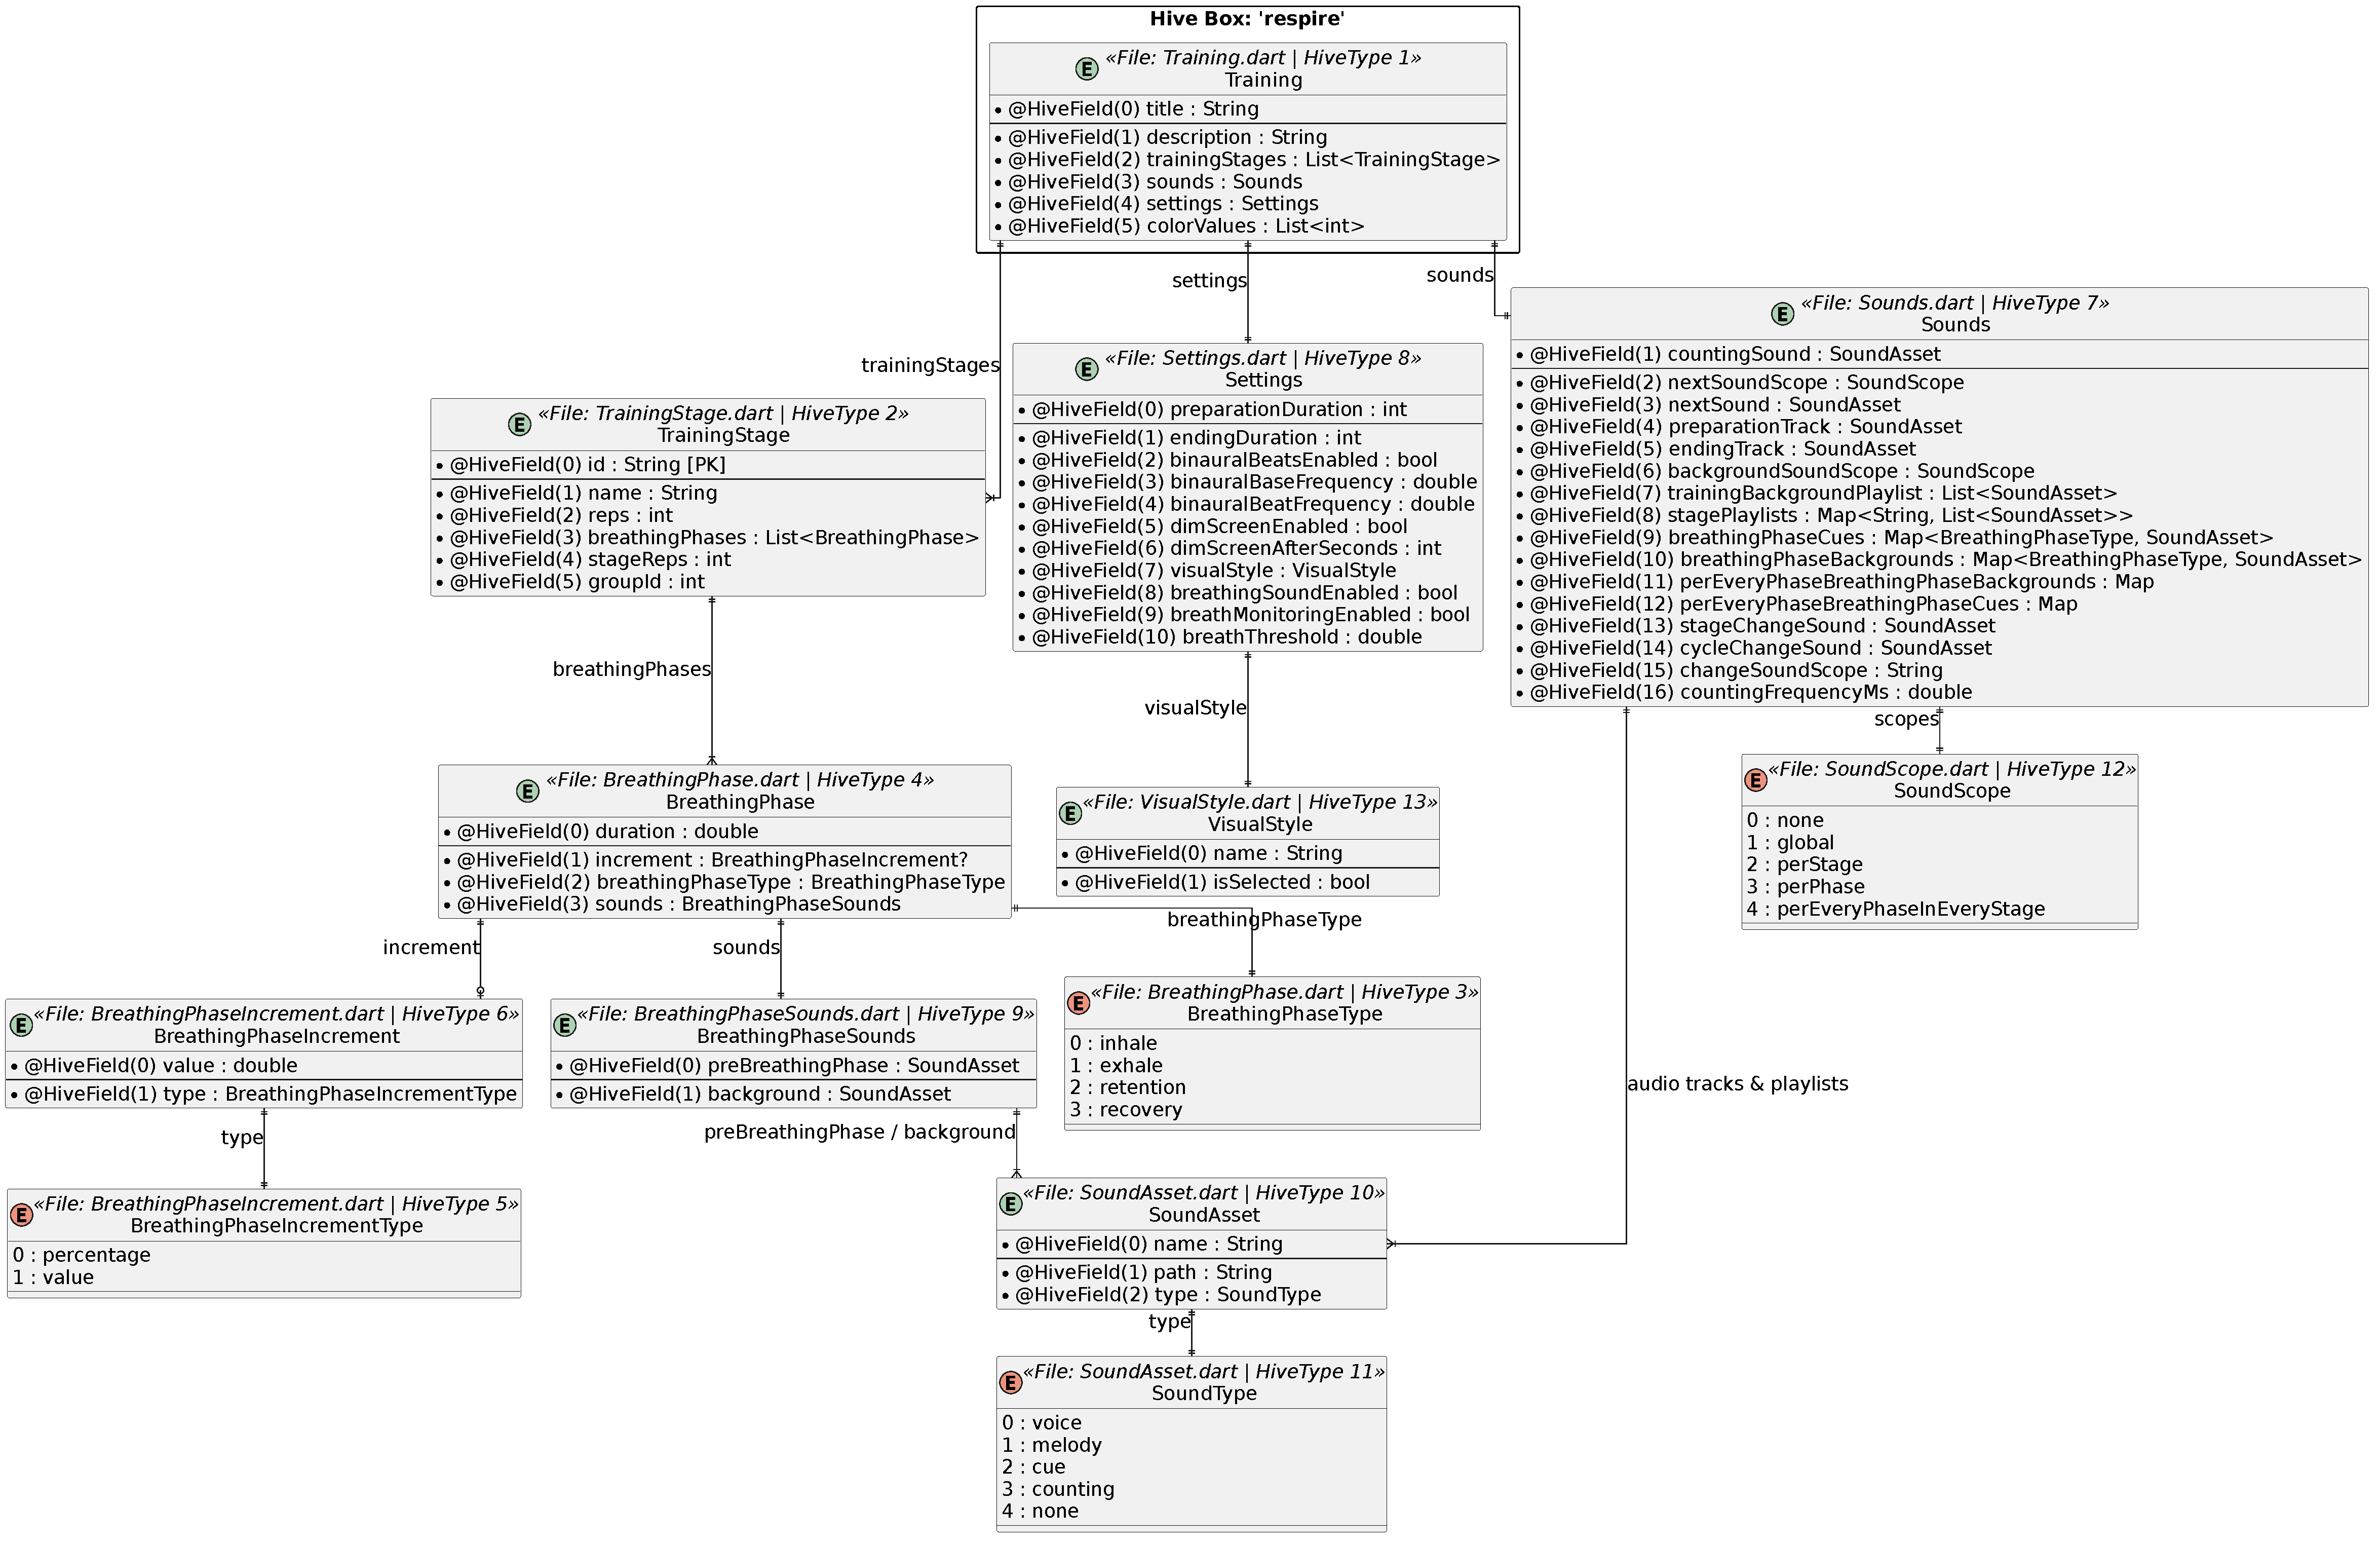
\includegraphics[width=1.10\textheight,height=1.05\textwidth,keepaspectratio]{obrazy/erd-1.pdf}%
    }
    \caption{Schemat ERD lokalnej bazy danych aplikacji ReSpire}
    \label{fig:training_erd}
\end{figure}
\end{landscape}

\subsection{Układ plików w repozytorium projektu aplikacji}

Repozytorium aplikacji składa się z części natywnej przeznaczonej dla systemu Android, katalogu zasobów oraz właściwego kodu aplikacji Flutter. Katalog \texttt{android} zawiera konfigurację projektu i pliki wymagane do zbudowania wersji mobilnej. Zasoby obejmują animacje, tłumaczenia, dźwięki i elementy graficzne, natomiast katalog \texttt{lib} przechowuje komponenty interfejsu, strony, usługi, motyw, funkcje pomocnicze oraz główny plik uruchamiający aplikację. Uproszczoną strukturę najważniejszych katalogów przedstawiono poniżej.

\dirtree{%
.1 android/.
.2 app/.
.3 src/.
.4 main/.
.3 build.gradle.
.2 gradle/.
.3 wrapper/.
.2 build.gradle.
.2 gradle.properties.
.2 settings.gradle.
.1 android/app/src/main/assets/.
.2 animations/.
.3 wave.json.
.2 languages/.
.3 en-US.json.
.3 pl-PL.json.
.2 sounds/.
.3 generator.dart.
.2 group\_logo.png.
.2 logo\_bez\_tla.png.
.1 lib/.
.2 components/.
.3 BreathingPage/.
.3 Global/.
.3 HomePage/.
.3 Settings/.
.3 TrainingEditorPage/.
.2 pages/.
.3 BreathingPage.dart.
.3 HomePage.dart.
.3 ProfilePage.dart.
.3 SettingsPage.dart.
.3 TrainingEditorPage.dart.
.3 TrainingPage.dart.
.2 services/.
.3 SoundManagers/.
.3 TranslationProvider/.
.3 BinauralBeatGenerator.dart.
.3 SettingsProvider.dart.
.3 TrainingController.dart.
.3 TrainingImportExportService.dart.
.3 UserSoundsDataBase.dart.
.2 theme/.
.3 Colors.dart.
.2 utils/.
.3 DurationFormatter.dart.
.3 TextUtils.dart.
.2 main.dart.
}

\section{Model CNN-Transformer w PyTorch}

Model klasyfikujący został zaimplementowany w PyTorch \cite{pytorchDocs2026}. Bibliotekę tę wybrano jako nowoczesne rozwiązanie zapewniające swobodę implementacji i intuicyjny sposób definiowania modeli, a także dostępność gotowych elementów transformera oraz możliwość przeprowadzenia treningu, ewaluacji i eksportu w jednym środowisku.

Do rozwoju kodu modelu w języku Python, uruchamiania skryptów treningowych, jak również analizy wyników wykorzystano środowisko Visual Studio Code.

Wejściem modelu nie jest bezpośrednio pełne nagranie, lecz krótki fragment dźwięku przekształcony do spektrogramu mel. Zgodnie z konfiguracją udokumentowaną w repozytorium modelu wykorzystywana jest częstotliwość próbkowania 44,1 kHz, okna o długości 0,3 s oraz reprezentacja zawierająca 128 pasm mel \cite{breathingClassificationGithub2026}. Takie podejście zapewnia krótki czas reakcji i umożliwia bieżące wykrywanie wydechu podczas treningu.

Zastosowany model bazowy ma architekturę hybrydową CNN-Transformer. Spektrogram mel jest najpierw przetwarzany przez ekstraktor cech złożony z trzech warstw splotowych Conv2D oraz operacji redukujących wymiar częstotliwościowy. Uzyskane mapy cech są spłaszczane do sekwencji ramek czasowo-częstotliwościowych, rzutowane liniowo do wymiaru modelu i uzupełniane kodowaniem pozycyjnym. Tak przygotowana sekwencja trafia do enkodera transformera, po którym zastosowano warstwę dropout oraz w pełni połączoną głowicę wyjściową generującą predykcje dla kolejnych ramek. W aplikacji wynik modelu jest wykorzystywany wyłącznie do wykrywania wydechu. Podczas działania aplikacji rozpoznany wydech oznacza zakończenie cyklu oddechowego, a także stanowi podstawę do zwiększenia licznika.

Do aplikacji Flutter dołączany jest gotowy, wcześniej wytrenowany model zapisany w formacie ONNX. Podczas działania aplikacji jego architektura i wyuczone wagi nie są modyfikowane. Zmiana sposobu działania modelu wymaga przeprowadzenia ponownego treningu w środowisku Python, ponownego eksportu oraz zastąpienia pliku ONNX w zasobach aplikacji. Bez ponownego uczenia można regulować jedynie próg decyzyjny, na podstawie którego wynik modelu jest uznawany za wykrycie wydechu. Zmiana progu wpływa na czułość detekcji, która może wymagać dostosowania w zależności od używanego sprzętu.

\section{Eksport modelu do ONNX}

Model utworzony w PyTorch nie jest bezpośrednio dołączany do aplikacji. Po zakończeniu treningu jest przełączany w tryb ewaluacji i eksportowany do formatu ONNX. PyTorch udostępnia w tym celu moduł \texttt{torch.onnx}, który przekształca graf obliczeniowy do przenośnej reprezentacji \cite{pytorchOnnxExporter2026}. W katalogu modelu transformerowego służy do tego osobny skrypt \texttt{export\_to\_onnx.py} \cite{breathingClassificationGithub2026}.

ONNX pełni funkcję warstwy pośredniej pomiędzy środowiskiem treningowym a aplikacją. Format zapisuje strukturę grafu, operatory oraz parametry modelu, dzięki czemu wnioskowanie nie wymaga uruchamiania interpretera Pythona ani pełnego PyTorch \cite{onnxConcepts2026}. Plik jest umieszczany w~zasobach aplikacji, a następnie otwierany przez warstwę wykonawczą zgodną z ONNX Runtime. Środowisko to obsługuje wykonywanie modeli między innymi na systemie Android lub iOS \cite{onnxRuntimeMobile2026}.

Podczas integracji należy zachować zgodność wejścia modelu z przetwarzaniem zastosowanym w Pythonie. Dotyczy to częstotliwości próbkowania, długości okna, liczby pasm mel, kolejności wymiarów tensora, typu danych oraz normalizacji. Należy przy tym zachować szczególną ostrożność, ponieważ nawet poprawnie wyeksportowany model może zwracać błędne wyniki, jeżeli aplikacja przygotuje spektrogram w inny sposób niż kod użyty podczas treningu.

Weryfikacja eksportu polega na przekazaniu tych samych danych wejściowych do wersji PyTorch i ONNX, jak również porównaniu uzyskanych wartości. Różnice powinny mieścić się w tolerancji wynikającej z obliczeń zmiennoprzecinkowych. Następnie model jest testowany w pełnym potoku aplikacji, obejmującym pobranie dźwięku, przygotowanie cech, wnioskowanie oraz aktualizację interfejsu.

\section{Działanie aplikacji}

Po uruchomieniu treningu aplikacja uzyskuje dostęp do mikrofonu i rozpoczyna odbieranie próbek audio. Dane są gromadzone do momentu utworzenia okna o wymaganej długości. Następnie wykonywane jest przetwarzanie wstępne, a także obliczenie reprezentacji wejściowej. Tensor trafia do modelu ONNX, który zwraca wynik określający obecność wydechu w analizowanym fragmencie. Pełny przepływ przetwarzania sygnału, od pozyskania dźwięku do wyświetlenia informacji zwrotnej w interfejsie użytkownika, przedstawiono na rysunku \ref{fig:breath_flow_chart}.

\begin{figure}[H]
    \centering
    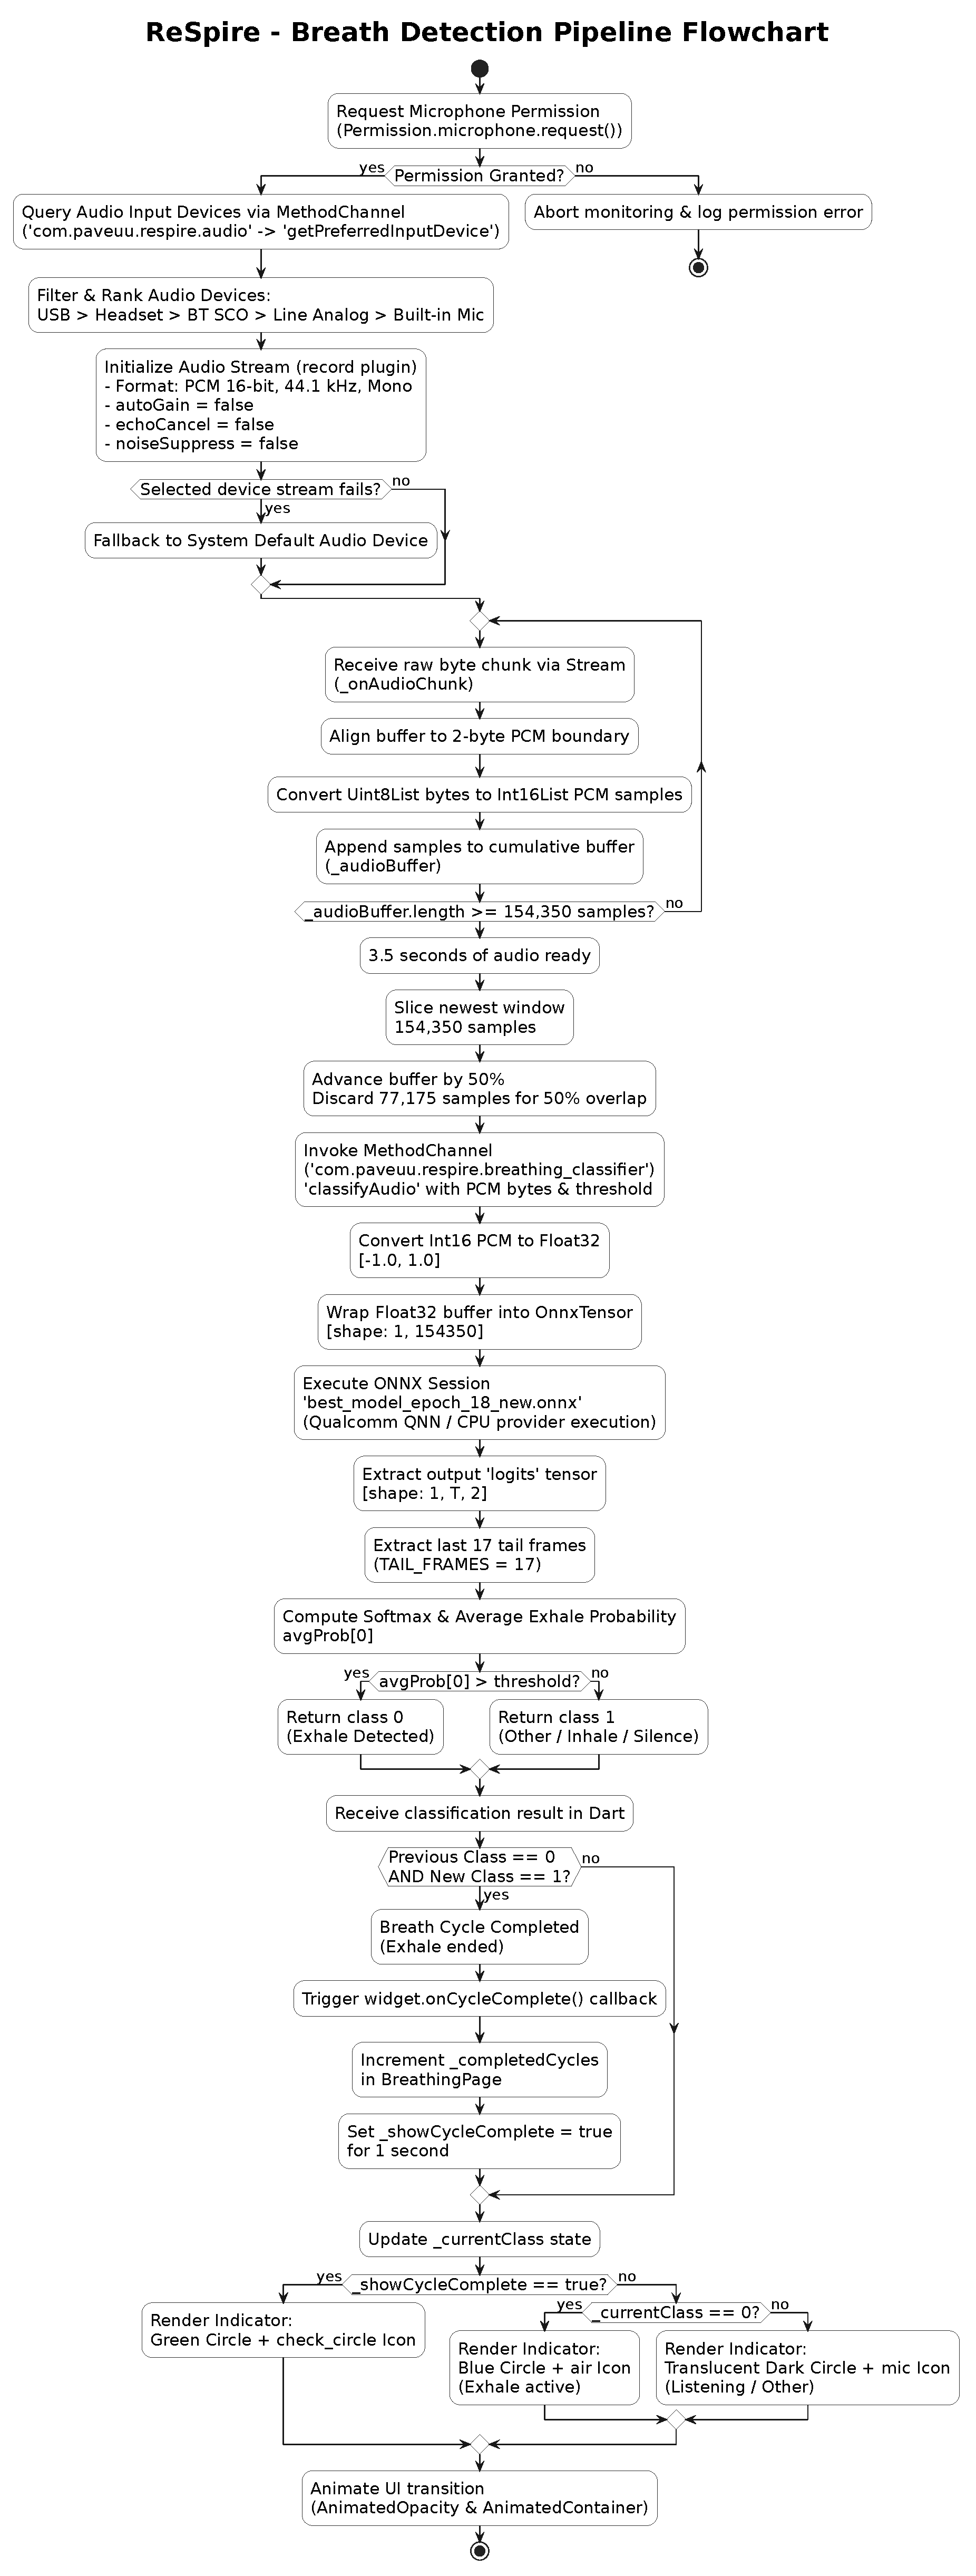
\includegraphics[width=0.95\linewidth,height=0.72\textheight,keepaspectratio]{obrazy/breath_flow_chart.pdf}
    \caption{Przepływ przetwarzania sygnału oddechowego od jego pozyskania do wyświetlenia informacji zwrotnej w interfejsie użytkownika}
    \label{fig:breath_flow_chart}
\end{figure}

Wynik detekcji jest przekazywany do interfejsu aplikacji. Rozpoznanie wydechu oznacza zakończenie bieżącego cyklu oddechowego i powoduje zwiększenie jego licznika. Proces jest powtarzany dla kolejnych fragmentów nagrania, dzięki czemu aplikacja może na bieżąco monitorować przebieg treningu. Implementacja modelu nie służy do pełnej klasyfikacji faz oddechu, lecz wyłącznie do identyfikowania wydechów potrzebnych do zliczania cykli.

Gdy model nie wykryje wydechu, licznik pozostaje bez zmian. Pozwala to pominąć wdechy, przerwy w treningu oraz fragmenty, które nie zawierają cech charakterystycznych dla wydechu.

\section{Iteracyjny proces rozwoju i dokumentacja}

Projekt był rozwijany iteracyjnie, a kolejne wersje kodu zapisywano w repozytorium GitHub. Każda większa zmiana mogła być analizowana jako osobny etap rozwoju: od modyfikacji interfejsu ReSpire, przez integrację modułu \texttt{exhale\_detection}, po zastosowanie transformera i eksport ONNX. Historia zmian umożliwiała porównywanie wariantów, odtwarzanie wcześniejszych wersji oraz wskazanie momentu wprowadzenia poszczególnych funkcji.

Projekt był rozwijany w dwóch oddzielnych repozytoriach, odpowiadających jego głównym warstwom. Repozytorium \textit{ReSpire} zawierało aplikację mobilną. Drugie repozytorium, \textit{breathing-classification-v3} obejmowało część związaną ze sztuczną inteligencją. Zawierało ono kod związany z  przygotowaniem i przetwarzaniem danych, implementację oraz trening modelu, jego ewaluację, jak również eksport do formatu ONNX. Rozdzielenie obu części umożliwiało niezależne rozwijanie aplikacji i modelu, przy zachowaniu jasno określonego sposobu ich integracji. Pozwoliło to zachować czytelność oraz porządek obu części.

\subsection{Zarządzanie zadaniami w Trello}

Do planowania prac i śledzenia postępu wykorzystano również narzędzie Trello. Tablica projektu stanowiła uzupełnienie systemu kontroli wersji. Umożliwiła ona organizowanie zadań związanych z rozwojem aplikacji. Poszczególne listy odpowiadały kolejnym wersjom systemu, a~umieszczone na nich karty opisywały planowane funkcje, poprawki interfejsu, zadania techniczne oraz wykryte problemy.

Taki sposób organizacji ułatwiał określenie zakresu kolejnych iteracji, a także kontrolowanie stopnia realizacji poszczególnych zmian. Po ukończeniu zadania jego stan był aktualizowany na tablicy, dzięki czemu możliwe było szybkie sprawdzenie, które elementy danej wersji zostały wykonane, a~które wymagały dalszej pracy. Ukończenie każdej owej listy było finalizowane zbudowaniem nowej wersji aplikacji. Przykładową postać tablicy wykorzystywanej podczas rozwoju aplikacji przedstawiono na rysunku \ref{fig:trello_board}.

\begin{figure}[H]
    \centering
    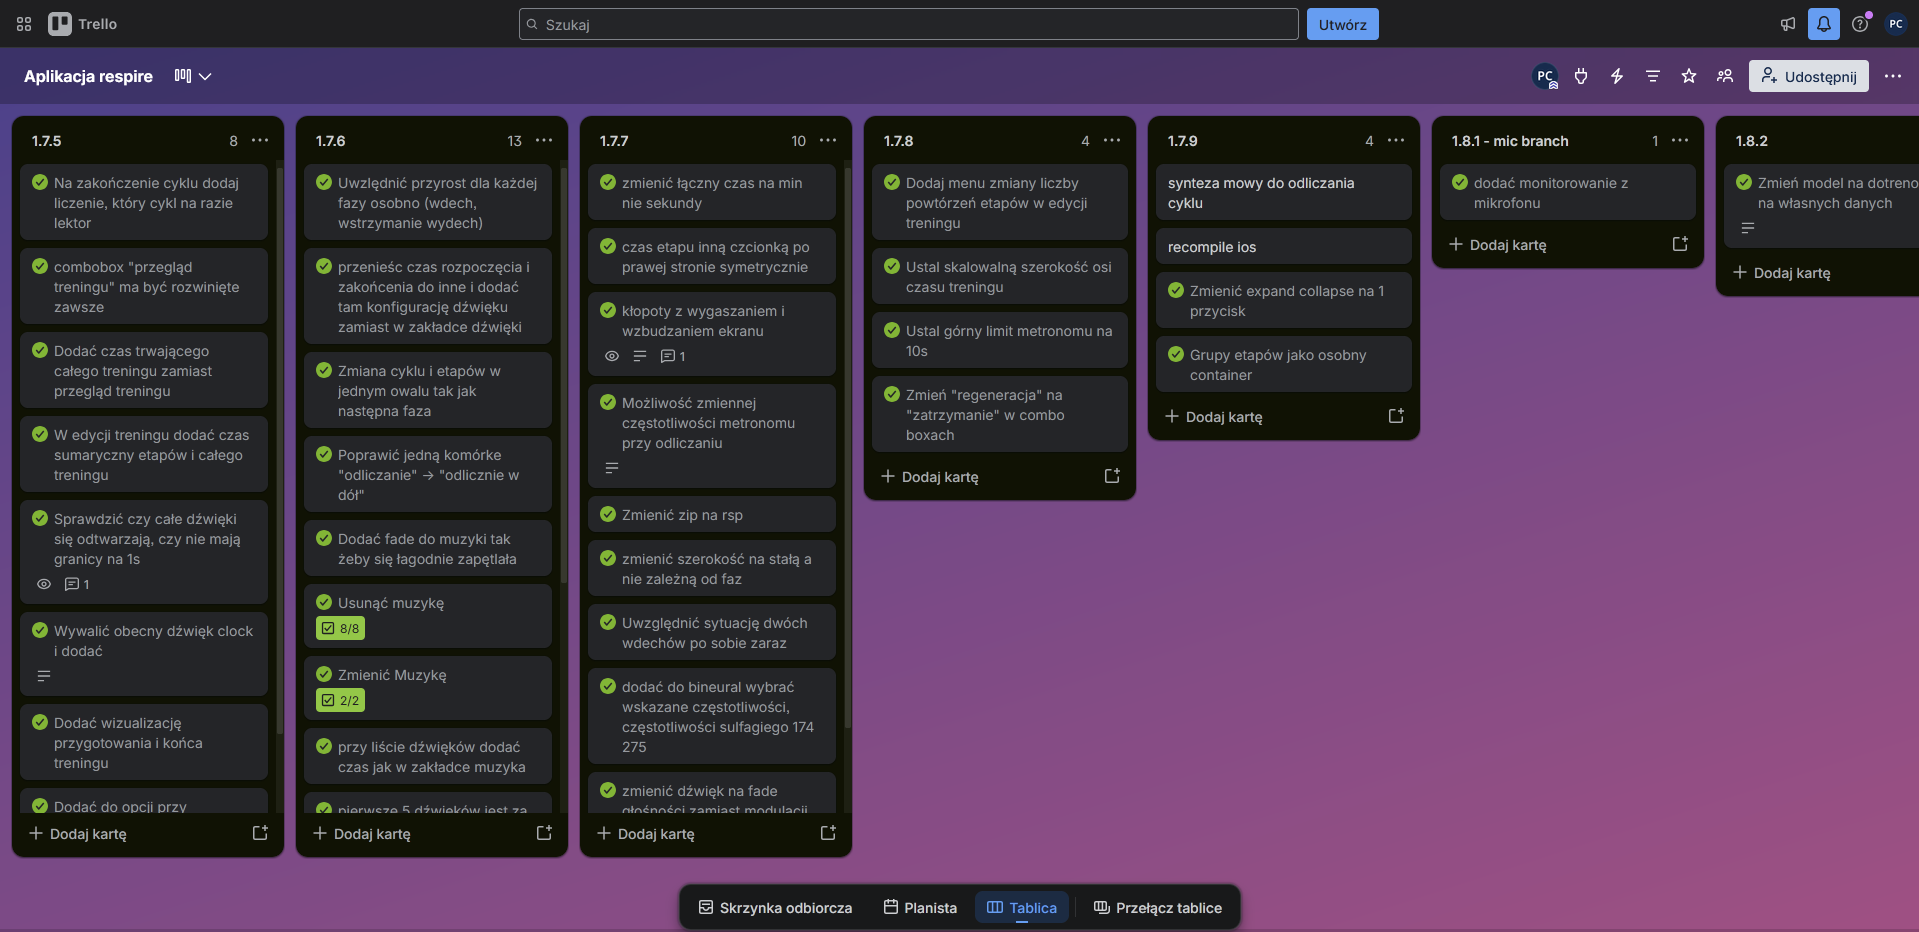
\includegraphics[width=\linewidth,height=0.72\textheight,keepaspectratio]{obrazy/trello-board.png}
    \caption{Tablica Trello wykorzystywana do zarządzania zadaniami i kolejnymi wersjami aplikacji}
    \label{fig:trello_board}
\end{figure}

\section{Podsumowanie}

Zaimplementowane rozwiązanie łączy wieloplatformową aplikację Flutter z modelem CNN-Transformer przygotowanym w PyTorch. Format ONNX oddziela środowisko treningowe od mobilnego środowiska wykonawczego i umożliwia integrację modelu bez osadzania Pythona w aplikacji. ReSpire dostarczył podstawę interfejsu. Projekt klasyfikacji oddechu, jak również moduł detekcji wydechu zapewniły natomiast punkt wyjścia dla analizy dźwięku oraz zliczania cykli na podstawie wykrytych wydechów.

Iteracyjny rozwój w repozytoriach GitHub umożliwił stopniowe udoskonalanie interfejsu, modelu i sposobu ich integracji. Przyjęta architektura pozostawia możliwość dalszego rozwijania każdej warstwy niezależnie, np. zastąpienia modelu nowszą wersją ONNX, dodania kolejnej platformy docelowej lub rozszerzenia aplikacji o historię treningów, a także dodatkowe formy wizualizacji.